

\section{Prueba 3}

\begin{comment}
R1: Si c Entonces h, FC=0.4
R2: Si c Entonces i, FC=0.75
R3: Si d Entonces i, FC=-0.4
R4: Si e Entonces h, FC=-0.55
R5: Si g y b Entonces i, FC=-0.1
R6: Si f Entonces h, FC=-0.6
\end{comment}
\subsection{Red de inferencia}
\begin{center}
	\tikzstyle{regla}= [rectangle,draw,black,fill=blue!15]
	\tikzstyle{hecho}= [rectangle,draw,black,fill=black!15]
	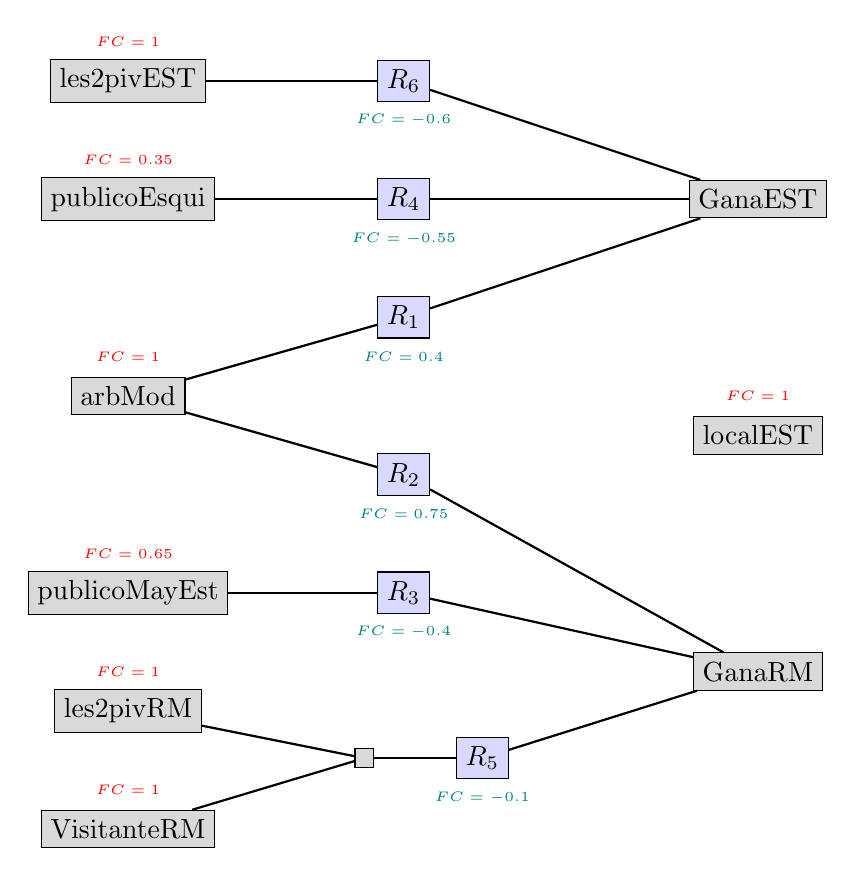
\begin{tikzpicture}
			
		\node (a) at (8,6.5) [hecho] {localEST};
		\node at (8,7) {\color{red}{\tiny{$FC=1$}}};

		\node (b) at (0,1.5) [hecho] {VisitanteRM};
		\node at (0,2) {\color{red}{\tiny{$FC=1$}}};

		\node (c) at (0,7) [hecho] {arbMod};
		\node at (0,7.5) {\color{red}{\tiny{$FC=1$}}};

		\node (d) at (0,4.5)[hecho] {publicoMayEst};
		\node at (0,5) {\color{red}{\tiny{$FC=0.65$}}};

		\node (e) at (0,9.5)[hecho] {publicoEsqui};
		\node at (0,10) {\color{red}{\tiny{$FC=0.35$}}};

		\node (f) at (0,11)[hecho] {les2pivEST};
		\node at (0,11.5) {\color{red}{\tiny{$FC=1$}}};

		\node (g) at (0,3)[hecho] {les2pivRM};
		\node at (0,3.5) {\color{red}{\tiny{$FC=1$}}};

		\node (h) at (8,9.5)[hecho] {GanaEST};

		\node (i) at (8,3.5)[hecho] {GanaRM};

		\node (g/b) at (3,2.4)[hecho] {};

		\node (r1) at (3.5,8) [regla] {$R_{1}$};
		\node at (3.5,7.5) {\color{teal}{\tiny{$FC=0.4$}}};
		\node (r2) at (3.5,6) [regla] {$R_{2}$};
		\node at (3.5,5.5) {\color{teal}{\tiny{$FC=0.75$}}};
		\node (r3) at (3.5,4.5) [regla] {$R_{3}$};
		\node at (3.5,4) {\color{teal}{\tiny{$FC=-0.4$}}};
		\node (r4) at (3.5,9.5) [regla] {$R_{4}$};
		\node at (3.5,9) {\color{teal}{\tiny{$FC=-0.55$}}};
		\node (r5) at (4.5,2.4) [regla] {$R_{5}$};
		\node at (4.5,1.9) {\color{teal}{\tiny{$FC=-0.1$}}};
		\node (r6) at (3.5,11) [regla] {$R_{6}$};
		\node at (3.5,10.5) {\color{teal}{\tiny{$FC=-0.6$}}};

		\path[black,thick] (f) edge[] node {} (r6);
		\path[black,thick] (r6) edge[] node {} (h);
		\path[black,thick] (e) edge[] node {} (r4);
		\path[black,thick] (r4) edge[] node {} (h);
		\path[black,thick] (c) edge[] node {} (r1);
		\path[black,thick] (r1) edge[] node {} (h);

		\path[black,thick] (c) edge[] node {} (r2);
		\path[black,thick] (r2) edge[] node {} (i);
		\path[black,thick] (d) edge[] node {} (r3);
		\path[black,thick] (r3) edge[] node {} (i);
		\path[black,thick] (g) edge[] node {} (g/b);
		\path[black,thick] (b) edge[] node {} (g/b);
		\path[black,thick] (g/b) edge[] node {} (r5);
		\path[black,thick] (r5) edge[] node {} (i);

	\end{tikzpicture}
\end{center}

\subsection{Objetivo obtenido por SBR-FC}

\subsection{Cuestión}
\begin{ejer}
	\textbf{Prueba 3.} ¿Quién ganará este tercer partido y, por tanto, la liga?
\end{ejer}